% Architecture v0.1 -- generated by tools/gen_architecture.py (same layout as the .drawio file)
\documentclass[tikz,border=2mm]{standalone}
\usepackage[T1]{fontenc}
\usepackage[scaled=0.92]{helvet}
\renewcommand{\familydefault}{\sfdefault}
\usepackage{textcomp}
\usetikzlibrary{arrows.meta,calc,positioning}

\definecolor{cred}{HTML}{E30613}
\definecolor{credfill}{HTML}{FDEBEC}
\definecolor{cdark}{HTML}{222222}
\definecolor{cgray}{HTML}{666666}
\definecolor{cline}{HTML}{D0D0D0}
\definecolor{clanelocal}{HTML}{F6F6F6}
\definecolor{clanecloud}{HTML}{EEF3FA}
\definecolor{clanecloudline}{HTML}{C9D6E8}
\definecolor{cblue}{HTML}{4A6FA5}
\definecolor{cwhite}{HTML}{FFFFFF}
\definecolor{cinfra}{HTML}{F5F5F5}

\begin{document}
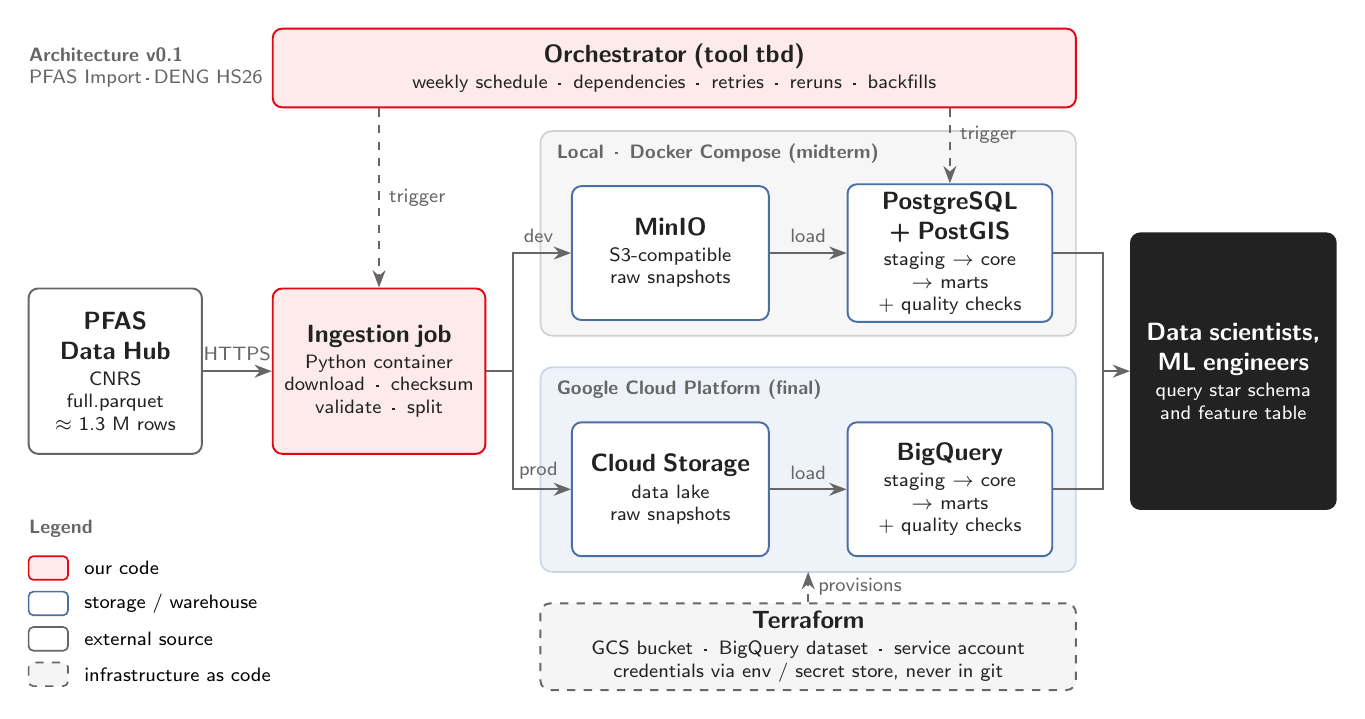
\begin{tikzpicture}[x=1mm,y=-1mm,
  box/.style={draw, rounded corners=1.2mm, line width=0.7pt, align=center, inner sep=1mm},
  lbl/.style={font=\scriptsize, text=cgray},
  arr/.style={-{Stealth[length=2.2mm]}, line width=0.7pt, draw=cgray},
  darr/.style={arr, dashed},
  font=\small]

\draw[rounded corners=1.5mm, fill=clanelocal, draw=cline, line width=0.6pt] (65,13) rectangle (133,39);
\node[anchor=north west, font=\scriptsize\bfseries, text=cgray, inner sep=0] at (67,14.6) {Local \,\textperiodcentered\, Docker Compose (midterm)};
\draw[rounded corners=1.5mm, fill=clanecloud, draw=clanecloudline, line width=0.6pt] (65,43) rectangle (133,69);
\node[anchor=north west, font=\scriptsize\bfseries, text=cgray, inner sep=0] at (67,44.6) {Google Cloud Platform (final)};
\node[box, fill=credfill, draw=cred, text=cdark, minimum width=102mm, minimum height=10mm, text width=100mm, font=\scriptsize] (orch) at (82.0,5.0) {{\small\bfseries Orchestrator (tool tbd)\par}\vspace{0.5mm}weekly schedule \,\textperiodcentered\, dependencies \,\textperiodcentered\, retries \,\textperiodcentered\, reruns \,\textperiodcentered\, backfills};
\node[box, fill=cwhite, draw=cgray, text=cdark, minimum width=22mm, minimum height=21mm, text width=20mm, font=\scriptsize] (src) at (11.0,43.5) {{\small\bfseries PFAS Data Hub\par}\vspace{0.5mm}CNRS\\full.parquet\\$\approx$ 1.3 M rows};
\node[box, fill=credfill, draw=cred, text=cdark, minimum width=27mm, minimum height=21mm, text width=25mm, font=\scriptsize] (ing) at (44.5,43.5) {{\small\bfseries Ingestion job\par}\vspace{0.5mm}Python container\\download \,\textperiodcentered\, checksum\\validate \,\textperiodcentered\, split};
\node[box, fill=cwhite, draw=cblue, text=cdark, minimum width=25mm, minimum height=17mm, text width=23mm, font=\scriptsize] (minio) at (81.5,28.5) {{\small\bfseries MinIO\par}\vspace{0.5mm}S3-compatible\\raw snapshots};
\node[box, fill=cwhite, draw=cblue, text=cdark, minimum width=26mm, minimum height=17mm, text width=24mm, font=\scriptsize] (pg) at (117.0,28.5) {{\small\bfseries PostgreSQL + PostGIS\par}\vspace{0.5mm}staging $\rightarrow$ core\\$\rightarrow$ marts\\+ quality checks};
\node[box, fill=cwhite, draw=cblue, text=cdark, minimum width=25mm, minimum height=17mm, text width=23mm, font=\scriptsize] (gcs) at (81.5,58.5) {{\small\bfseries Cloud Storage\par}\vspace{0.5mm}data lake\\raw snapshots};
\node[box, fill=cwhite, draw=cblue, text=cdark, minimum width=26mm, minimum height=17mm, text width=24mm, font=\scriptsize] (bq) at (117.0,58.5) {{\small\bfseries BigQuery\par}\vspace{0.5mm}staging $\rightarrow$ core\\$\rightarrow$ marts\\+ quality checks};
\node[box, fill=cdark, draw=cdark, text=cwhite, minimum width=26mm, minimum height=35mm, text width=24mm, font=\scriptsize] (cons) at (153.0,43.5) {{\small\bfseries Data scientists, ML engineers\par}\vspace{0.5mm}query star schema\\and feature table};
\node[box, fill=cinfra, draw=cgray, text=cdark, minimum width=68mm, minimum height=11mm, text width=66mm, font=\scriptsize, dashed] (tf) at (99.0,78.5) {{\small\bfseries Terraform\par}\vspace{0.5mm}GCS bucket \,\textperiodcentered\, BigQuery dataset \,\textperiodcentered\, service account\\credentials via env / secret store, never in git};
\coordinate (fork) at (61.5,43.5);
\coordinate (join) at (136.5,43.5);

\draw[arr] (src.east) -- node[above, lbl] {HTTPS} (ing.west);
\draw[line width=0.7pt, draw=cgray] (ing.east) -- (fork);
\draw[arr] (fork) |- node[pos=0.72, above, lbl] {dev} (minio.west);
\draw[arr] (fork) |- node[pos=0.72, above, lbl] {prod} (gcs.west);
\draw[arr] (minio) -- node[above, lbl] {load} (pg);
\draw[arr] (gcs) -- node[above, lbl] {load} (bq);
\draw[line width=0.7pt, draw=cgray] (pg.east) -| (join);
\draw[line width=0.7pt, draw=cgray] (bq.east) -| (join);
\draw[arr] (join) -- (cons.west);
\draw[darr] (orch.south -| ing.north) -- node[right, lbl] {trigger} (ing.north);
\draw[darr] (orch.south -| pg.north) -- node[right, lbl, pos=0.35] {trigger} (pg.north);
\draw[darr] (tf.north) -- node[right, lbl] {provisions} (tf.north |- 0,69);

\node[anchor=west, font=\scriptsize\bfseries, text=cgray, inner sep=0] at (0,63.5) {Legend};
\draw[rounded corners=0.6mm, fill=credfill, draw=cred, line width=0.6pt] (0,67.0) rectangle (5,70.0);
\node[anchor=west, font=\scriptsize, inner sep=0] at (7,68.5) {our code};
\draw[rounded corners=0.6mm, fill=cwhite, draw=cblue, line width=0.6pt] (0,71.5) rectangle (5,74.5);
\node[anchor=west, font=\scriptsize, inner sep=0] at (7,73.0) {storage / warehouse};
\draw[rounded corners=0.6mm, fill=cwhite, draw=cgray, line width=0.6pt] (0,76.0) rectangle (5,79.0);
\node[anchor=west, font=\scriptsize, inner sep=0] at (7,77.5) {external source};
\draw[rounded corners=0.6mm, fill=cinfra, draw=cgray, line width=0.6pt, dashed] (0,80.5) rectangle (5,83.5);
\node[anchor=west, font=\scriptsize, inner sep=0] at (7,82.0) {infrastructure as code};
\node[anchor=west, align=left, font=\scriptsize, text=cgray, inner sep=0] at (0,5) {\textbf{Architecture v0.1}\\PFAS Import\,\textperiodcentered\,DENG HS26};
\end{tikzpicture}
\end{document}
